\documentclass[letterpaper,10 pt,conference]{ieeeconf}

\IEEEoverridecommandlockouts
\overrideIEEEmargins

\usepackage[utf8]{inputenc}
\usepackage[T1]{fontenc}

\usepackage{graphics} % for pdf, bitmapped graphics files
%\usepackage{mathptmx} % assumes new font selection scheme installed
\usepackage{times} % assumes new font selection scheme installed
\usepackage{amsmath} % assumes amsmath package installed
\usepackage{amssymb}  % assumes amsmath package installed


\usepackage{graphics} % for pdf, bitmapped graphics files
\usepackage{caption}
\usepackage{subcaption}
\usepackage{standalone}
\usepackage{tikz}
\usepackage{tikzscale}
\usetikzlibrary{calc}

\graphicspath{{img/}}

\title{\LARGE \bf
  Optimizing Topometric Maps for Teach and Repeat
}


\author{David Landry and Alexandre Gari\'epy}


\begin{document}

\maketitle
\thispagestyle{empty}
\pagestyle{empty}


\begin{abstract}

  abstract

\end{abstract}

\section{INTRODUCTION}



\begin{itemize}
    \item Talk about teach and repeat
    \item How teach maps are aquired (point clouds are taken at regular steps)
    \item Why we want to optimize this (loop closure spped, memory for large maps)
\end{itemize}


\section{RELATED WORK}


\section{PROBLEM DEFINITION}

We begin with an unoptimized topometric map, containing $N$ a set of interconnected nodes and $T$
the geometric transformations to go from one node to it's neighbor. The nodes in $N$ are in fact
anchor points to our teach an repeat implementation. They are point clouds in this case, but could
be any mean of localization, like features in an image. Every node $n_i$ has an associated point
cloud $p_i$. The nodes are linked as a chain, from the first node recorded to the last.

Our objective is to find the smallest subset of $N$ such that the robot can reliably localize itself
against a node at any time while it follows the taught trajectory. To decide wether the robot can
localize itself at a given position in the global frame, we will induce an error in the
transformation estimate between both nodes. The intuition behind it is that by inducing increasingly
large errors, we can guarantee an increasingly large robustness by going in the field. At some point
the localisation will fail: the ICP algorithm will enter a local minimum, and the result of the ICP
will be largely different that the induced error.
\section{OUR APPROACH}
\label{approach}

\begin{itemize}
  \item Choose elipse of a given shape. We assume that if ICP converges on the
    ellipse, it would converge at any given point inside the ellipse (we need the explain why we made this assumption)

  \item For each point, find the nearest point that doesn't converge with ICP

  \item Create an oriented graph where arcs represents a successful ICP convergence

  \item Find the shortest path in the graph from that converge

\end{itemize}

\begin{figure}[thpb]
  \centering
  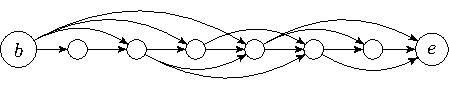
\includegraphics[scale=1.0]{unoptimized-graph}
  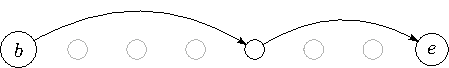
\includegraphics[scale=1.0]{optimized-graph}
  \caption{Optimal node subset using the graph approach}
\end{figure}


\section{EXPERIMENTS}
We can talk about the offline optimisation we did on some dataset.

\begin{figure}
  \centering
  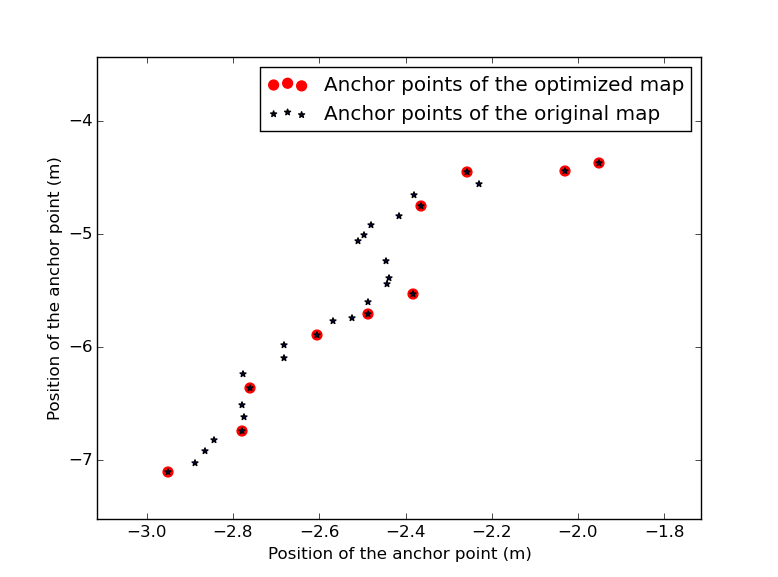
\includegraphics[scale=0.4]{map_optimization}
  \caption{Comparison of un-optimized and optimized maps}
\end{figure}

We tested the algorithm on a few datasets that were recorded through previous \textit{teach}
sessions. Our approach was indeed able to greatly reduce the number of anchor points needed to
localize a \textit{repeat} session.

We noticed that the \textit{ICP chain} used to reconstruct the relative positions between the nodes
may be noisier than we thought, yielding unrealistic positions for sucessive anchor points. It
leaves us wondering wether we should rather rely on the odometry from the weels as a reference
transformation.

\begin{table}[h]
\centering
\begin{tabular}{|l|r|r|r|}
  \hline
Dataset & N. of points & N. of points after optimization & \% \\
\hline
terasse & 304 & 186 & 61.2 \\
  \hline
\end{tabular}
\caption{The result of the optimization on different datasets}

\end{table}

\section{FUTURE WORK}

\begin{itemize}
  \item Experiment with Husky
\end{itemize}

\subsection{Multi-objective optimization for automatic parameter selection}

To focus our efforts on fiding the minimal node subset, we made the simplication the error ellipse has a fixed sized.
In other words, we manually specify the distance in $x$ and $y$ for which we want the ICP to converge. With those parameters given,
we can reduce the problem to a finding the shortest path in a graph, as shown in section \ref{approach}.


A limitation of this approach is that, if for a given node, decreasing the size of the ellipse would make the ICP
converge on further nodes of the graph. We can see that as a tradeoff between the precision and the number of nodes of the final map.


An improvement on the current method would be model the problem as a multi-objective optimization problem. Given an initial
ellipse size for each node of the graph, changing reducing the size of the ellipse has a cost. The goal is to find the best
tradeoff between the length of the shortest path in the graph and the the costs of the nodes that are used by that shortest path.

\subsection{Handling of rotations}

For the sake of simplicity we did not use rotations when inducing errors to the reading's
position estimate, before testing the reliability of the localization. To make the optimization
problem more difficult, while giving the user more ways garantee the reliability of the optimized
maps, we could replace $T$ the space of translations with $R \times T$ the space of rotations and
translations in function $f$. That way, the user could demand that the generated maps be tolerant to
a certain error in the orientation of the robot.

Using the whole space of rotations $R$ might be too general, as it is often useful to simplify the pose of a
ground robot begin a vector $[x, y, \theta]^t$, $\theta$ being the heading. That case could also be
handled by replacing the tolerance ellipse by an ellipsoid. The supplementary dimension would
represent the error in heading, or $\Delta \theta$.

\subsection{Reoptimization of the localizability graph}



\section{CONCLUSION}

\end{document}
